% *******************************************************************************
% * Copyright (c) 2007 by Elexis
% * All rights reserved. This document and the accompanying materials
% * are made available under the terms of the Eclipse Public License v1.0
% * which accompanies this distribution, and is available at
% * http://www.eclipse.org/legal/epl-v10.html
% *
% * Contributors:
% *    G. Weirich - initial implementation
% *
% *  $Id: rest.tex 2933 2007-07-29 10:05:35Z rgw_ch $
% *******************************************************************************
% !Mode:: "TeX:UTF-8" (encoding info for WinEdt)

\section{'Views' divers}

\subsection{Affichage des données}
Cette 'View' permet d'afficher des multiples champs de la base de données de Elexis. Plusieurs exemplaires de cette 'View' (avec du contenu identique ou variable) peuvent être intégrés dans une perspective.  (cf Fif. \ref{figure1}).
\begin{figure}[hb]
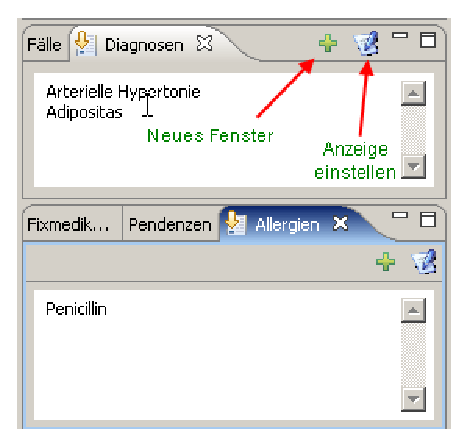
\includegraphics{images/data1}
\caption{Zwei Fenster der 'Datenanzeige'}
\label {figure1}
\end{figure}
En cliquant sur le bouton- \textbf{+} vous pouvez ouvrir un exemplaire supplémentaire de cette 'View' , en cliquant sur le bouton pour éditer vous pouvez ajuster les données à afficher.

\begin{figure}[hb]
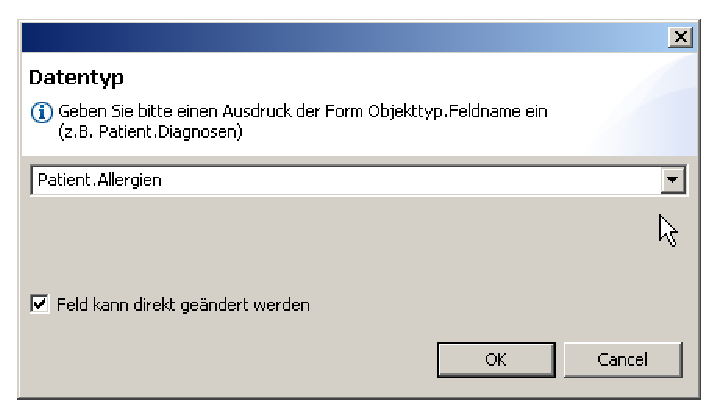
\includegraphics{images/data2}
\caption{Eingabedialog für den Datentyp}
\label{figure2}
\end{figure}
Il apparaîtra une boite de dialogue comme montré dans Fig. \ref{figure2}.
Vous pouvez introduire ici chaque type de données qui peut également être utilisé comme variable dans des présentations de texte (cf page \pageref{Platzhalter}).
Si vous activez la case 'champ peut être modifié' (à condition que vous avez les droits pour ceci) les donnés peuvent être modifiés directement en écrivant dans cette fenêtre. L'arrangement et le contenu des 'affichages de données' sont sauvegardés lors de la fermeture de Elexis ou lors de l'action 'sauvegarde de perspective'.



\subsection{Médication fixe}
Cette 'View' montre la médication fixe du patient sélectionné actuellement (cf Fig. \ref{fig:fixmedi})

\begin{figure}[htp]
\begin{center}
  \includegraphics{images/fixmediview}
  \caption{Fixmedikation}
  \label{fig:fixmedi}
\end{center}
\end{figure}
Vous pouvez tirer les médicaments depuis la fenêtre des articles ou depuis une ordonnance directement dans cette 'View' et vous pouvez aussi tirer des articles depuis la médication fixe dans une ordonnance. Par un clic sur  \glqq ajouter\ldots\grqq{} ouvrez la 'View'-articles.  En cliquant sur \glqq liste\ldots\grqq{} vous créez un plan de traitement pour le patient. Pour ceci il doit exister une présentation de texte nommée \glqq plan de traitement\grqq{}
et celle-ci doit contenir quelque part la variable [liste des médicaments]. En cliquant sur  \glqq ordonnance\grqq{} vous créez une ordonnance contenant la médication régulière du patient. Pour ceci doit exister une présentation de texte nommée\glqq ordonnance\grqq qui contient quelque part une variable [lignes d'ordonnance].

\subsection{Historique de la médication }
Cette 'View' montre tous les médicaments, qui ont jamais été prescrits ou donnés au patient actuel, avec date et dosage (si mentionné). En cliquant sur les en-têtes des différentes colonnes vous pouvez ordonner la liste selon date de remise ou selon nom du médicament. Pour les médicaments qui font partie de la médication fixe il y a aura en outre (si c'est précisé) mention de la date d'arrêt du médicament.

\subsection{Compendium online}
Si vous avez une connexion Internet active vous voyez dans cette 'View' le compendium Suisse des médicaments . 

\subsection{Open Drug Database}
Lorsque vous avez une connexion Internet active, cette 'View' affiche  le site correspondant que vous pouvez utiliser pour la recherche des génériques ou des interactions médicamenteuses.

\subsection{Affaires pendantes}
Rappels, Reminders, affaires pendantes : Cette 'View' affiche les choses dont vous aimeriez ou vous devriez vous souvenir (cf Fig. \ref{fig:pendenzen}).

\begin{wrapfigure}{l}{7.5cm}
  \includegraphics[width=7.2cm]{images/pendenzenview}
  \caption{Pendenzen-View}
  \label{fig:pendenzen}
\end{wrapfigure}

Une affaire pendante a une date d'échéance et un état (planifié, vient à l'échéance, en retard, réglé, reste inachevé).

l y a les types suivants d'affaires pendantes :
\begin{itemize}
  \item Devoirs pour une personne ou devoirs pour tous.
  \item Rappels qui s'affichent toujours lorsque la date d'échéance est atteinte ou dépassée. 
  \item Rappels qui s'affichent seulement lorsque la date d'échéance est atteinte 
  \textit{et} si un patient spécifique est affiché..
  \item Affaires pendantes qui ne sont pas seulement affichées mais qui déclenchent aussi une action spécifique (par ex. écrire une lettre en série)
\end{itemize}

Le symbole des affaire pendantes s'affiche dans la liste des patients (cf Fig. \ref{fig:pendenzen})si des affaires pendantes concernent un patient.

Pour créer une nouvelle 'affaire pendante' cliquez sur le symbole  \glqq nouvelle affaire pendante\grqq{}(boutton vert avec Plus blanc). Une boite de dialogue apparaîtra dans laquelle vous pouvez introduire un texte, choisir le type d'affaire pendante, la personne responsable, la date de l'échéance et l'état de l'affaire pendante.
 
Un double-clic sur une affaire pendante suffit pour ouvrir celle-ci pour la modifier. Il apparaît la même boite de dialogue.

